\documentclass{fenicscourse}

\begin{document}

\fenicslectureoverview{Anders Logg}{Chalmers, Dec 17--18 2012}

\begin{frame}
  \frametitle{Course outline}

  % Note to lecturers: use \textcolor{grey}{Lecture title} to mark
  % lectures that are not included in a course

  % Course plan
  %
  % Mon 2012-12-17 10-12, lunch, 13-16 5 hours
  % Tue 2012-12-16 10-12, lunch, 13-16 5 hours
  % Total: 10 hours
  %
  % Monday
  %
  % 10-12
  %
  %   --- This overview                30min
  %   L02 Static linear PDEs           1h 30min (challenge, coffee mug to winner(s))
  %
  % 13-16
  %
  %   L06 Static hyperelasticity       2h  (challenge, coffee mug to winner(s))
  %   L07 Dynamic hyperelasticity      2h  (leave implementation as homework)
  %
  % Tuesday
  %
  % 10-12
  %
  %   L08 The Stokes problem           2h  (no challenge)
  %   L05 Happy hacking                1h
  %   L09 Incompressible Navier-Stokes 2h  (challenge, coffee mug to winner(s))

  \small

  \begin{enumerate}
  \item[L00]
    \textcolor{grey}{Introduction to FEM}
  \item[L01]
    \textcolor{grey}{Introduction to FEniCS}
  \item[L02]
    Static linear PDEs (Monday)
  \item[L03]
    \textcolor{grey}{Static nonlinear PDEs}
  \item[L04]
    \textcolor{grey}{Time-dependent PDEs}
  \item[L05]
    Happy hacking: Tools, tips and coding practices (Tuesday)
  \item[L06]
    Static hyperelasticity (Monday)
  \item[L07]
    Dynamic hyperelasticity (Monday)
  \item[L08]
    The Stokes problem (Tuesday)
  \item[L09]
    Incompressible Navier--Stokes (Tuesday)
  \item[L10]
    \textcolor{grey}{Discontinuous Galerkin methods for elliptic equations}
  \item[L11]
    \textcolor{grey}{A posteriori error estimates and adaptivity}
  \end{enumerate}

  \normalsize

  {\footnotesize Lectures can be downloaded from
    \url{http://fenicsproject.org/pub/course/}}
\end{frame}


% The quickest FEniCS intro
\begin{frame}
\medskip

\includegraphics[width=0.99\textwidth]{png/fenics_banner.png}
\begin{columns}[c]
\begin{column}{0.4\textwidth}
\bf{The FEniCS Project is a collection of open-source software
  components aimed at the numerical solution of partial differential
  equations using finite element methods}
\end{column}
\begin{column}{0.7\textwidth}
  \begin{block}{Key distinguishing features}
  \begin{itemize}
  \item
    FEniCS (Python/C++) code is quick to write and easy to read
  \item
    `Any' finite element formulation of 'any' partial differential
    equation can be coded
  \item
    Automated code generation is heavily used under the hood to
    create efficient, specialized, low-level code
  \item
    Performance -- implicit problems with over $12\, 000\, 000\, 000$
    degrees of freedom can be solved in a couple of minutes
  \end{itemize}
  \end{block}
\end{column}
\end{columns}
  \begin{center}
    \colemph{\url{http://fenicsproject.org/}}
  \end{center}
\end{frame}

\begin{frame}
\frametitle{FEniCS has been used for a wide range of
  equations and applications}

{\tiny Reaction-diffusion equations; Stokes with or without nonlinear
  viscosity; compressible and incompressible Navier--Stokes; RANS
  turbulence models; shallow water equations; Bidomain equations;
  nonlinear and linear elasticity; nonlinear and linear
  viscoelasticity; Schr\"odinger; Biot's equations for porous media,
  fracture mechanics, electromagnetism, liquid crystals including
  liquid crystal elastomers, combustion, ... and coupled systems of
  the above, ...}

\begin{center}
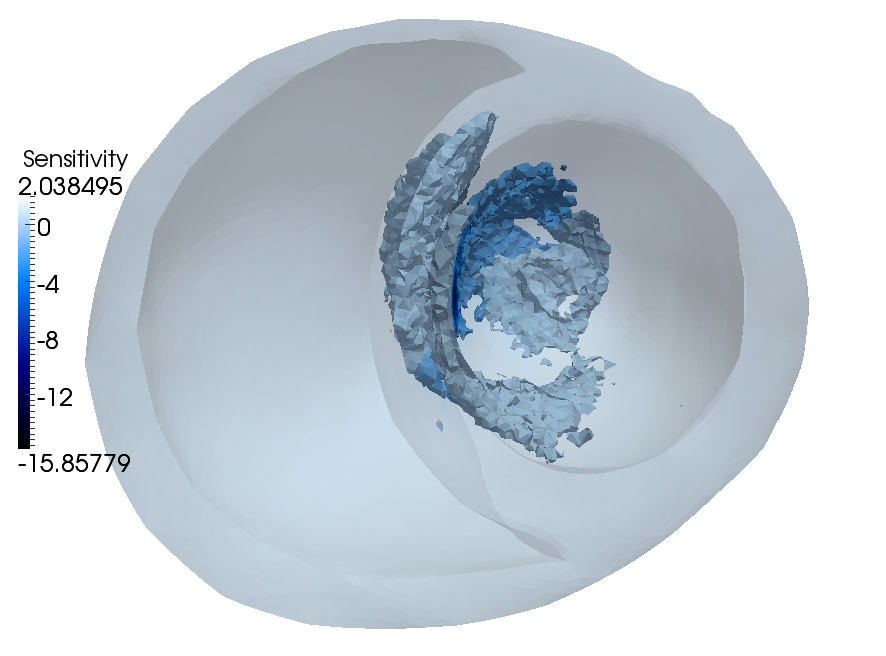
\includegraphics[width=0.24\textwidth]{png/g_el_plusx.png}
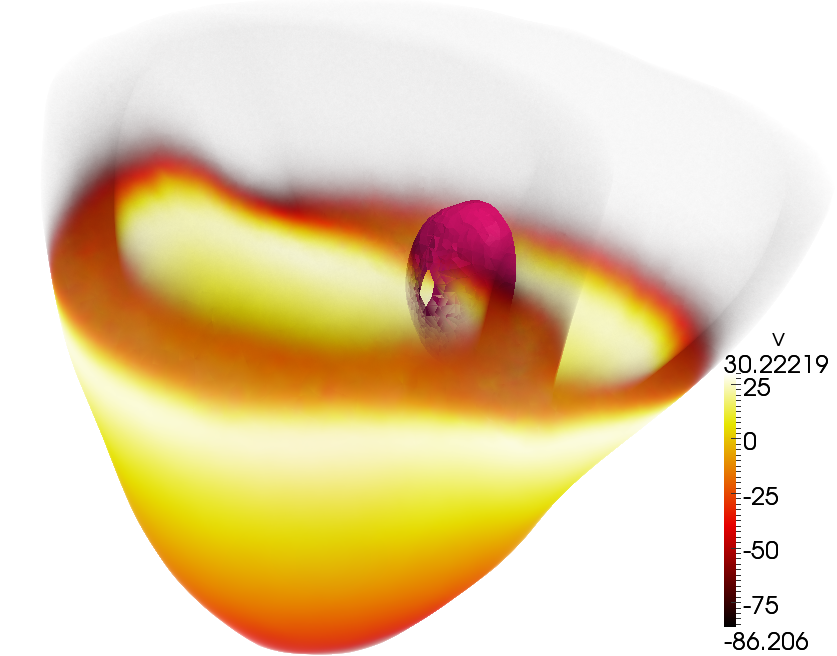
\includegraphics[width=0.24\textwidth]{png/unhealthy_v_at_T200.png}
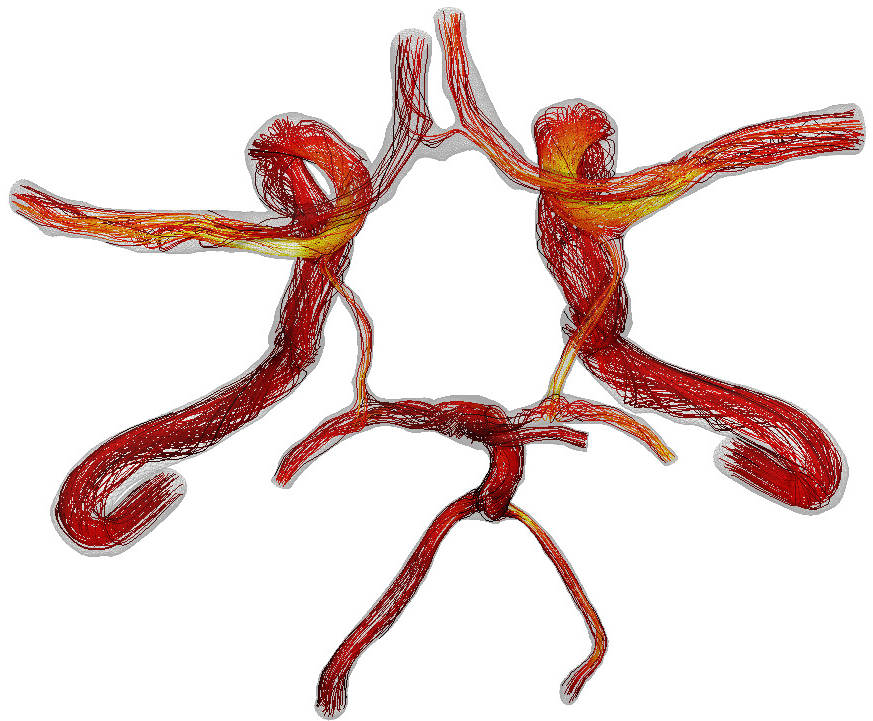
\includegraphics[width=0.24\textwidth]{png/circle_of_willis_simulation.png}
\end{center}

{\tiny for simulating blood flow, computing calcium release in cardic
  tissue, computing the cardiac potential in the heart, simulating
  mantle convection, simulating melting ice sheets, computing the
  optimal placement of tidal turbines, simulating and reconstructing
  tsunamis, simulating the flow of cerebrospinal fluid and the
  deformation of the spinal cord, simulating waveguides, ... }

\end{frame}


% Learning more than what this course covers
\begin{frame}
    \frametitle{Sounds great, but how do I find my way through the
    jungle?}
    \begin{center}
        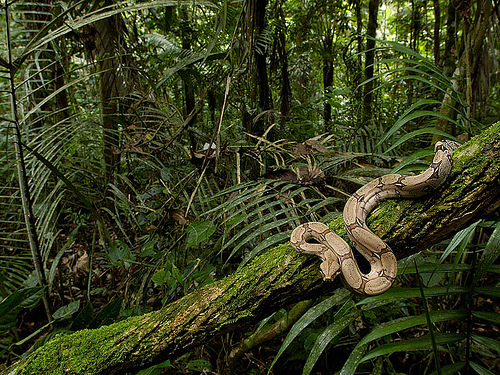
\includegraphics[width=0.8\textwidth]{jpg/jungle10.jpg}
    \end{center}
\end{frame}

\begin{frame}
    \frametitle{Three survival advices}
    \begin{columns}[c]
        \begin{column}{0.33\textwidth}
            \begin{center}
                
\includegraphics[width=0.99\textwidth]{png/python_logo.png}
            \end{center}
        \end{column}
        \begin{column}{0.33\textwidth}
            \begin{center}
                
\includegraphics[width=0.99\textwidth]{jpg/documentation.jpg}\\
            \end{center}
        \end{column}
        \begin{column}{0.33\textwidth}
            \begin{center}
                
\includegraphics[width=0.99\textwidth]{jpg/question-blue.jpg}
            \end{center}
        \end{column}
    \end{columns}
    \begin{columns}[t]
        \begin{column}{0.33\textwidth}
            \begin{center}
                \colemph{Use the right Python tools}
            \end{center}
        \end{column}
        \begin{column}{0.33\textwidth}
            \begin{center}
                \colemph{Explore the documentation}
            \end{center}
        \end{column}
        \begin{column}{0.33\textwidth}
            \begin{center}
                \colemph{Ask, report and request}
            \end{center}
        \end{column}
    \end{columns}
\end{frame}


% TODO: Update webpage images when readthedocs work is completed

% Demos on old page
\begin{frame}
  \begin{center}
     {
\includegraphics[width=0.80\textwidth]{png/fenics-doc-webpage-5.png}}
    \small
    \colemph{\url{http://fenicsproject.org/documentation/}}
  \end{center}
\end{frame}

% Reference docs on old page
\begin{frame}
  \begin{center}
     {
\includegraphics[width=0.80\textwidth]{png/fenics-doc-webpage-6.png}}
    \small
    \colemph{\url{http://fenicsproject.org/documentation/}}
  \end{center}
\end{frame}

% Currently migrating
\begin{frame}
  \begin{center}
     {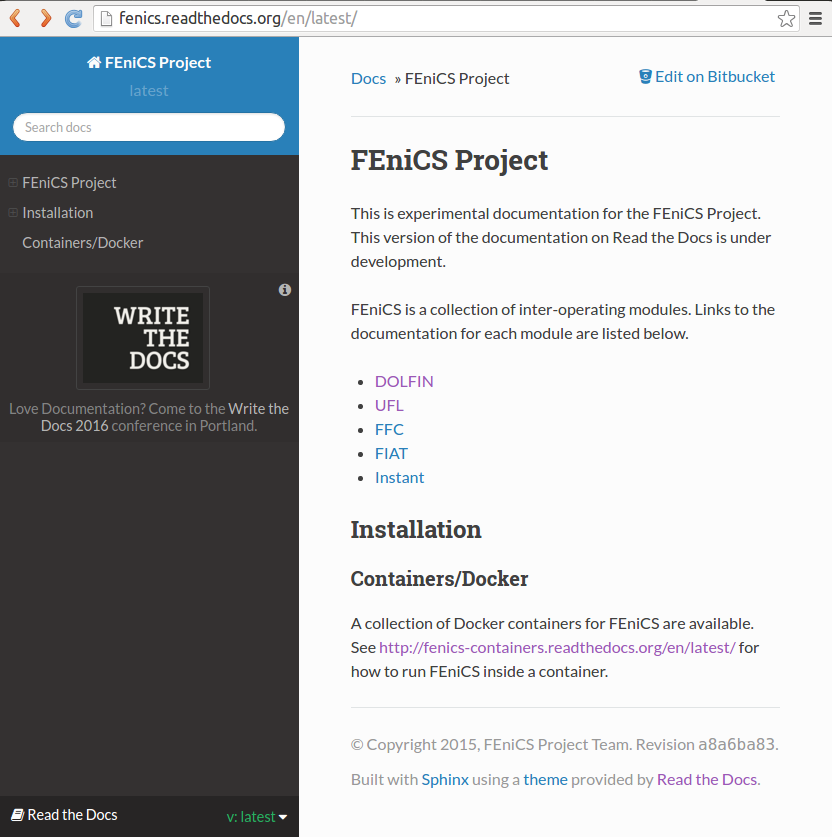
\includegraphics[width=0.80\textwidth]{png/fenics-readthedocs-webpage-1.png}}
    \small
    \colemph{\url{http://fenics.readthedocs.org/}}
  \end{center}
\end{frame}

\begin{frame}
    \frametitle{Development community is organized via bitbucket.org}
    \begin{center}
        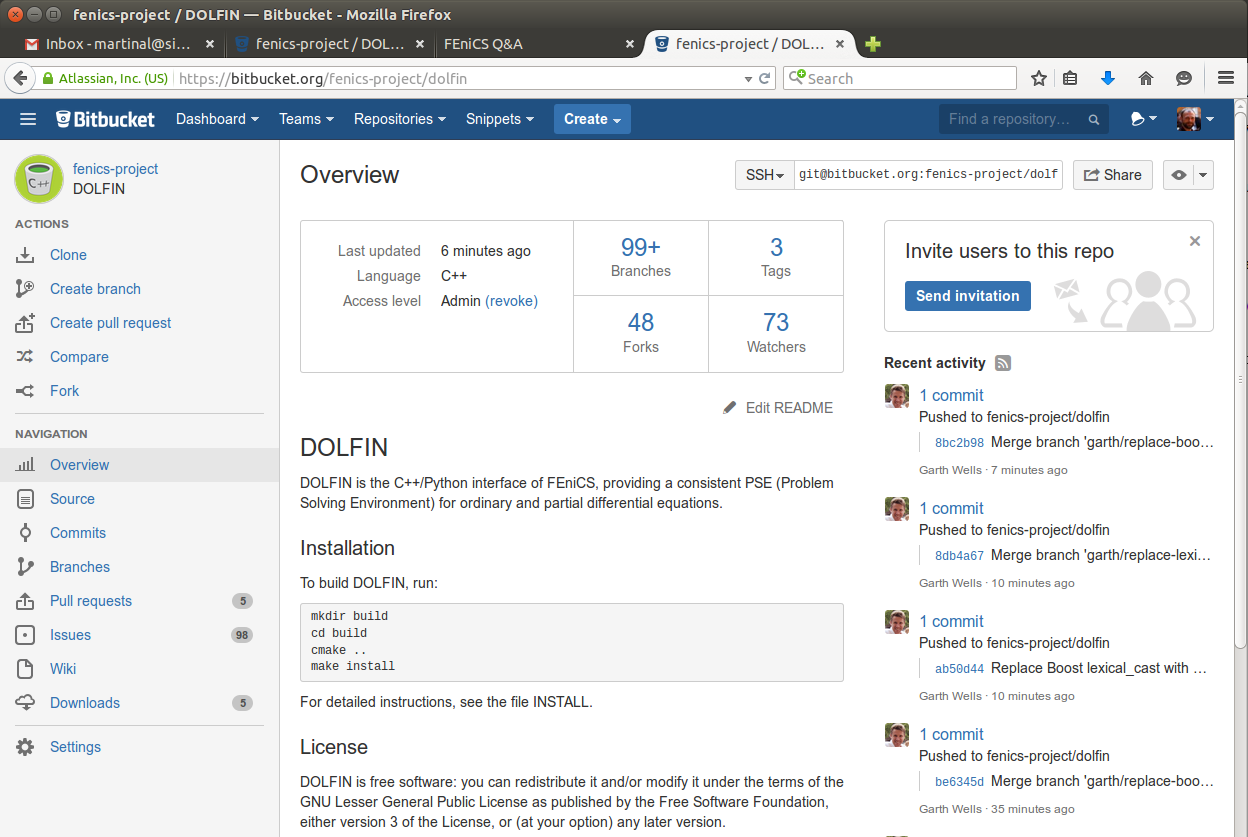
\includegraphics[height=0.75\textheight]{png/fenics-bitbucket-webpage.png}
        \vspace{1em}
        \small
        \colemph{\url{http://bitbucket.org/fenics-project/}}
    \end{center}
\end{frame}
\begin{frame}
    \frametitle{Community help is available via QA forum}
    \begin{center}
        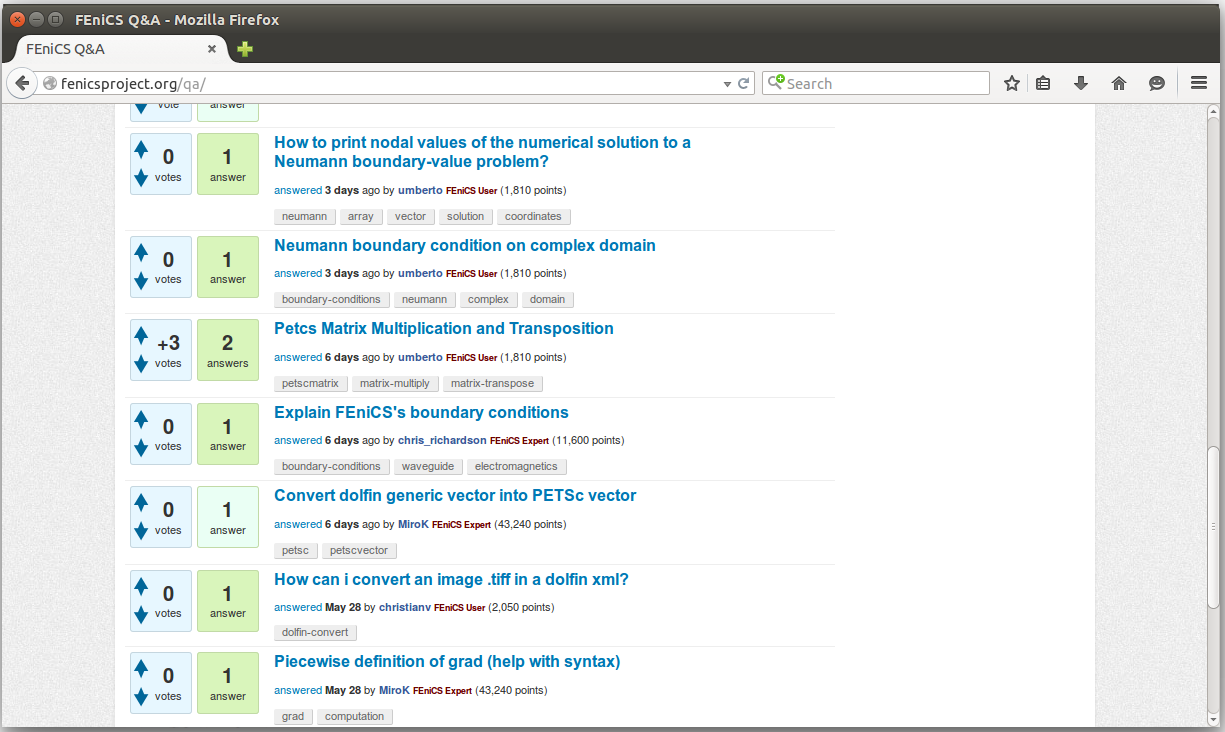
\includegraphics[width=1.0\textwidth,height=0.7\textheight]{png/fenics-qa-website.png}
        \vspace{1em}
        \small
        \colemph{\url{https://fenicsproject.org/qa}}
    \end{center}
\end{frame}


\begin{frame}
  \frametitle{Installation alternatives}

  % FEniCS uses standard setup.py and cmake tools
  % but dependencies are tricky to configure.

  \begin{tabular}{cp{10cm}}
    
\includegraphics[height=1cm]{png/docker_logo.png} &
    \begin{minipage}{10cm}
      \ding{43} Docker images on Linux, Mac, Windows
      \vspace{0.6cm}
    \end{minipage}
    \\
    
\includegraphics[height=1cm]{png/source.png} &
    \begin{minipage}{10cm}
      \ding{43} Build from source with Hashdist (fenics-install.sh)
      \vspace{0.8cm}
    \end{minipage}
    \\
    
\includegraphics[height=1cm]{png/ubuntu_logo.png} &
    \begin{minipage}{10cm}
      \ding{43} PPA with apt packages for Debian and Ubuntu
      \vspace{0.6cm}
    \end{minipage}
    \\
    
\includegraphics[height=1cm]{png/mac_osx_logo.png} &
    \begin{minipage}{10cm}
      \ding{43} Drag and drop installation on Mac OS X
      \vspace{0.8cm}
    \end{minipage}
  \end{tabular}

  \begin{center}
    \colemph{\url{http://fenicsproject.org/download/}}
  \end{center}

\end{frame}


\begin{frame}{Let's get started and remember:}

\linespread{2.0}
\bigskip
\begin{itemize}
\item
{\footnotesize \textbf{Lectures} can be downloaded from
  \url{http://fenicsproject.org/pub/course/lectures}}

\item
{\footnotesize \textbf{Data} for exercises can be downloaded from
  \url{http://fenicsproject.org/pub/course/data}}

\item
{\footnotesize \textbf{Solutions} for exercises can be downloaded from
  \url{http://fenicsproject.org/pub/course/src} \\
(Secret password needed!)
}
\end{itemize}
\linespread{1.0}\

\end{frame}

\end{document}
